\section{System Design and Methodology}
\label{sec:methodology}

\subsection{Objectives and scope}

The system was designed around five objectives: (i) scenarios should be explicit and machine-validated; (ii) execution should use real container network stacks and standard Linux tools; (iii) routing and impairment state should be checked rather than assumed; (iv) each run should produce structured, traceable evidence; and (v) extensions should reuse the same bounded execution path. The system is an experimental NDT, not a synchronized replica of a production network. Its supported claims concern controlled behaviour and workflow reproducibility within evaluated configurations.

\begin{figure}[t]
\centering
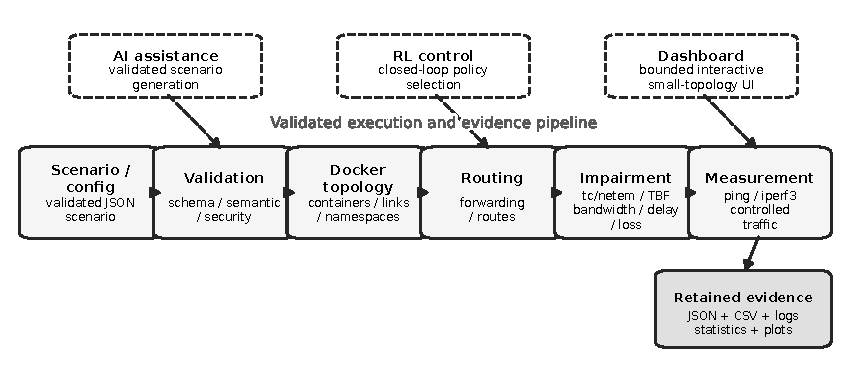
\includegraphics[width=\linewidth]{figures/architecture/overall_system_architecture.pdf}
\caption{Overall architecture. Scenario validation, Docker execution, routing, impairment, measurement, and evidence retention form the core pipeline. AI assistance, RL control, and the Dashboard are bounded extensions rather than independent core systems.}
\label{fig:architecture}
\end{figure}

Figure~\ref{fig:architecture} summarizes the execution path. A scenario/configuration enters validation before any topology is built. The validated representation drives Docker topology creation, routing and forwarding, impairment configuration, and measurement. Results are serialized as JSON/CSV and accompanied where available by logs, summaries, statistics, and plots. Cleanup is scoped to project-owned resources so that a failed run does not justify broad container or network deletion.

\subsection{Scenario representation and validation}

Scenarios describe topology identity, node roles, links, addressing, impairments, and traffic endpoints. Small experiments use allowlisted direct, routed, or two-router forms; the generic topology path supports larger graphs. Validation is layered. Schema checks reject malformed structures and unexpected fields. Semantic checks enforce unique identifiers, valid endpoints, bounded numeric parameters, and consistent links. For AI-originated content, prompt constraints and a projection stage further remove operational freedom: generated output cannot select arbitrary commands, images, credentials, or host paths. This makes validation a security boundary as well as a correctness check.

\subsection{Docker topology and routing}

Nodes are implemented as Docker containers attached to deterministic Docker networks. Routers enable forwarding; endpoints and routers receive addresses derived from the scenario. Direct scenarios require no intermediate route, while routed and multi-router scenarios install explicit paths and verify expected reachability. The generic topology path constructs a network per link and provisions routes required by the selected traffic pair. Route checks are retained with run evidence, avoiding the inference that container creation alone implies end-to-end connectivity.

Germany50 extends this mechanism using imported Topology Zoo data. The normalized scenario contains 50 router nodes and 88 links with deterministic subnets. Two routing modes were retained. Selected mode installs the routes needed for the three representative endpoint pairs. Full mode generates the theoretical 4,224-entry plan, but the retained full-mode evidence is a dry-run validation only. This separation is fundamental: plan generation, route installation, and traffic exercise are distinct claims.

\subsection{Impairment and measurement pipeline}

Linux traffic control implements the configured conditions. Token-bucket filtering (TBF) constrains bandwidth, while \texttt{netem} introduces one-way delay and packet loss. The framework records qdisc state where available and then executes ping and reverse TCP iperf3 traffic. Ping provides sent/received counts, loss, and RTT; iperf3 provides measured throughput. Configured one-way delay is therefore never relabelled as measured latency, and configured one-way loss is not equated with measured end-to-end loss.

Each run writes its normalized scenario and metrics into a run-specific directory. Batch runners add manifests, per-run rows, summaries, environment records, and cleanup outcomes. Failed or retried attempts remain visible. The dissertation inventory identifies which values were already repository-reported and which statistics were recomputed during a read-only audit.

\subsection{Automation extensions}

\paragraph{AI-assisted generation.} The AI path requests a structured scenario, validates it, projects it into the executable representation, and permits only dry-run or controlled execution. Provider identity is retained separately from validation outcome. The official OpenAI call and the OpenAI-compatible Qwen call therefore constitute different evidence items.

\paragraph{Closed-loop control.} The RL extension uses a minimal dual-path Docker topology. At each episode the controller observes measured network state, selects a path, verifies routing, runs ping and iperf3, computes reward, and checkpoints the outcome. Q-learning is compared with a threshold heuristic and two fixed-path policies under the same ordered two-phase schedule. The design tests whether learning can operate on real Docker measurements; it does not assume that learning is the best policy.

\paragraph{Dashboard.} The zero-dependency interactive server exposes allowlisted small-topology experiments on loopback. It supports validation, dry-run lifecycle, a confirmed direct real-Docker path, restricted downloads, and scoped cleanup. Germany50 and RL results remain read-only, and arbitrary Docker commands are not accepted. Because raw UI-path and regression/security logs were not retained, Dashboard evidence is used conservatively.

\subsection{Reproducibility and security}

Reproducibility is supported by versioned scenarios, runner scripts, per-run metrics, summaries, figures, failure records, and documentation. It does not mean that every environment will produce identical timing: Docker shares the host kernel and traffic-control timing is host-sensitive. Security measures include input allowlists, semantic bounds, separation of provider responses from execution, local-only Dashboard operation, argument-list Docker invocation, and project-scoped resource names. The retained repository does not contain the claimed raw fresh-clone, 69-test, secret-scan, or security-scan logs; this absence is reported rather than reconstructed.
